% Digital Logic Report Template
% Created: 2020-01-10, John Miller

%==========================================================
%=========== Document Setup  ==============================

% Formatting defined by class file
\documentclass[11pt]{article}

% ---- Document formatting ----
\usepackage[margin=1in]{geometry}	% Narrower margins
\usepackage{booktabs}				% Nice formatting of tables
\usepackage{graphicx}				% Ability to include graphics
\usepackage{multicol}

%\setlength\parindent{0pt}	% Do not indent first line of paragraphs 
\usepackage[parfill]{parskip}		% Line space b/w paragraphs
%	parfill option prevents last line of pgrph from being fully justified

% Parskip package adds too much space around titles, fix with this
\RequirePackage{titlesec}
\titlespacing\section{0pt}{8pt plus 4pt minus 2pt}{3pt plus 2pt minus 2pt}
\titlespacing\subsection{0pt}{4pt plus 4pt minus 2pt}{-2pt plus 2pt minus 2pt}
\titlespacing\subsubsection{0pt}{2pt plus 4pt minus 2pt}{-6pt plus 2pt minus 2pt}

% ---- Hyperlinks ----
\usepackage[colorlinks=true,urlcolor=blue]{hyperref}	% For URL's. Automatically links internal references.

% ---- Code listings ----
\usepackage{listings} 					% Nice code layout and inclusion
\usepackage[usenames,dvipsnames]{xcolor}	% Colors (needs to be defined before using colors)

% Define custom colors for listings
\definecolor{listinggray}{gray}{0.98}		% Listings background color
\definecolor{rulegray}{gray}{0.7}			% Listings rule/frame color

% Style for Verilog
\lstdefinestyle{Verilog}{
	language=Verilog,					% Verilog
	backgroundcolor=\color{listinggray},	% light gray background
	rulecolor=\color{blue}, 			% blue frame lines
	frame=tb,							% lines above & below
	linewidth=\columnwidth, 			% set line width
	basicstyle=\small\ttfamily,	% basic font style that is used for the code	
	breaklines=true, 					% allow breaking across columns/pages
	tabsize=3,							% set tab size
	commentstyle=\color{gray},	% comments in italic 
	stringstyle=\upshape,				% strings are printed in normal font
	showspaces=false,					% don't underscore spaces
}

% How to use: \Verilog[listing_options]{file}
\newcommand{\Verilog}[2][]{%
	\lstinputlisting[style=Verilog,#1]{#2}
}


%code to get a C-style 
\usepackage{xcolor}
\usepackage{listings}

\definecolor{mGreen}{rgb}{0,0.6,0}
\definecolor{mGray}{rgb}{0.5,0.5,0.5}
\definecolor{mPurple}{rgb}{0.58,0,0.82}
\definecolor{backgroundColour}{rgb}{0.95,0.95,0.92}

\lstdefinestyle{CStyle}{
	backgroundcolor=\color{backgroundColour},   
	commentstyle=\color{mGreen},
	keywordstyle=\color{magenta},
	numberstyle=\tiny\color{mGray},
	stringstyle=\color{mPurple},
	basicstyle=\footnotesize,
	breakatwhitespace=false,         
	breaklines=true,                 
	captionpos=b,                    
	keepspaces=true,                 
	numbers=left,                    
	numbersep=5pt,                  
	showspaces=false,                
	showstringspaces=false,
	showtabs=false,                  
	tabsize=2,
	language=C
}



%======================================================
%=========== Body  ====================================
\begin{document}

\title{ELC 4396 02 \\ Class Report 4}
\author{Jordan Cook}

\maketitle


\section{Introduction and Problem Statement} 

\quad The purpose of this coding project was to an aesthetically-pleasing night-light. There is a duo of RGB LED's found the Nexys4 DDR board. The goal was to create a pattern where the two lights would cycle through the rainbow, as well as have 4 different levels of brightness which would be controlled by two switches on the board. This would all be accomplished by utilizing pulse-width modulation.
\\\\ Link to the Project: \url{https://github.com/jordanstarr/System-on-Chip/tree/master/Class%20Report%204}

\section{Method and Approach}

\subsection{Hardware}

\quad The first step, as done in the previous report, was to create the FPGA itself. In order to do this, 16 files were downloaded from the textbook author's website (Dr. Pong Chu), as well as the constraint file necessary to program the Nexys board. Those files were: 

\begin{multicols}{2}
\begin{itemize}
	\item chu\_gpi.sv
	\item chu\_gpo.sv 
	\item chu\_timer.sv 
	\item fifo.sv 
	\item fifo\_ctrl.sv 
	\item reg\_file.sv
	\item chu\_mmio\_controller.sv 
	\item baud\_gen.sv 
	\item chu\_uart.sv 
	\item uart.sv 
	\item uart\_rx.sv 
	\item uart\_tx.sv 
	\item chu\_io\_map.sv 
	\item chu\_mcs\_bridge.sv 
	\item mmio\_sys\_vanilla.sv 
	\item mcs\_top\_vanilla.sv
\end{itemize}
\end{multicols} 

\quad With these files now included in the project, a CPU from the IP catalog was added to the project to ensure that everything would be working with any system updates.

\quad An additional file was needed to complete this: a pulse-width-modulation file. This was  provided by Dr. Pong Chu, which nothing was changed in his System Verilog code. It was connected to the FPGA like usual with other wrappers. In the top level file, an additional set of outputs were created that would connect the PWM to the two RGB lights. This was everything that was done on the hardware side. \\

\subsection{Software}
\quad From this point, an XSA file was exported and opened in the Vitis IDE. After going through the proper sections and creating a platform, certain files from Dr. Chu were needed to be added. These files were: 

\begin{multicols}{2}
	\begin{itemize}
		\item chu\_init
		\item chu\_init.h
		\item chu\_io\_map.h
		\item chu\_io\_rw.h
		\item gpio\_cores.cpp
		\item gpio\_cores.h
		\item timer\_core.cpp
		\item timer\_core.h
		\item uart\_core.cpp
		\item uart\_core.h
		\item main\_vanilla\_test.cpp		
	\end{itemize}
\end{multicols}

\quad Using classes already defined, a PWM and a GPI variable were created. The PWM would change the output of the colorful LED's and the GPI would provide data on how many of the switches were on (which would also be used as variable in the PWM output); 

\begin{lstlisting}[style=CStyle, caption = Core instantiations]
PwmCore myPwm(get_slot_addr(BRIDGE_BASE, S6_PWM));
GpiCore mySwitch(get_slot_addr(BRIDGE_BASE, S3_SW));
\end{lstlisting}

\quad A function was created in the rainbow function to determine which switches were high, which corresponds to how the maximum brightness of the LED's. Then based on which switches are flipped, a specific percentage is assigned that will be a multiplier later on. The original task was to set it in increments of 25\%, but for a more obvious change in brightness, it was redesigned to go from 5\%, to 30\%, to 65\%, and finally to full brightness. For debugging, the UART display function was needed to verify that the correct switches were being read (as seen in Putty).

\begin{lstlisting}[style=CStyle, caption = Switch Function]
double percent;
int switch1;
int switch2;
switch1 = sw_pointer -> read(0);
switch2 = sw_pointer -> read(1);

if (switch1 && switch2) {
	percent = 1.0;
}
else if (!switch1 && switch2) {
	percent = 0.65;
}
else if (switch1 && !switch2) {
	percent = 0.3;
}
else {
	percent = 0.05;
}

uart.disp("Percentage: ");
uart.disp(percent);
uart.disp("\n\r");
\end{lstlisting}

\quad Dr. Chu included some PWM code that would go through each of the three colors, get brighter, and change color. From this code, it was reverse-engineered to get a desired output for the use of this project. The following picture was also a huge aid in figuring out logic that would work: 

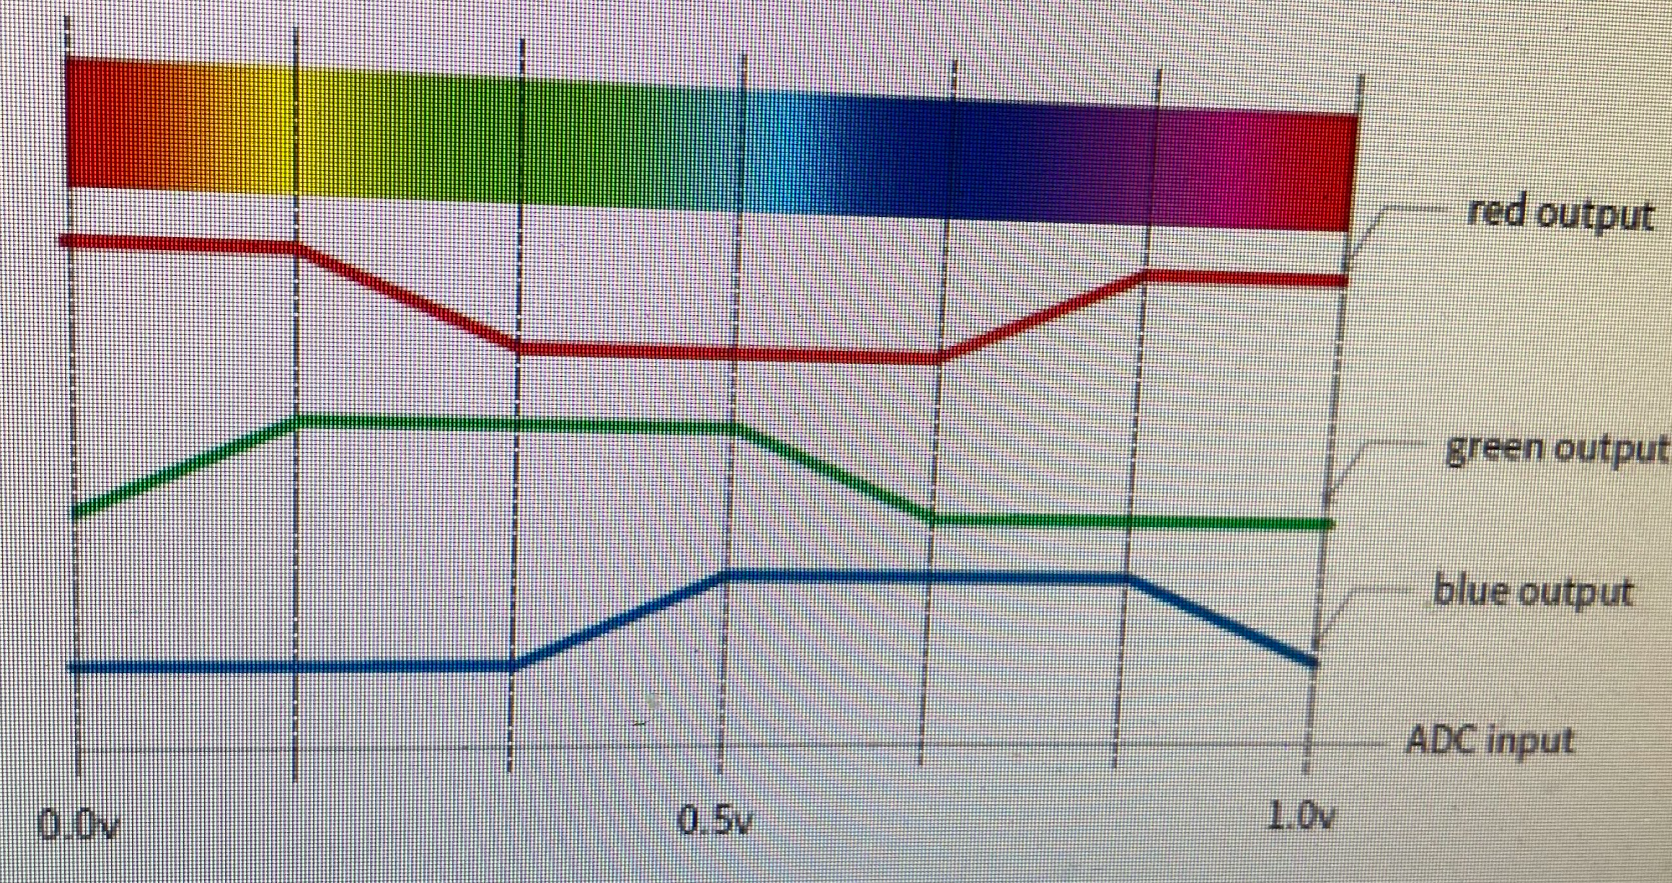
\includegraphics{RGB_scale}

\quad There were four actions that needed to be done: increase brightness, decrease brightness, set to maximum, or set to zero. This image could also be divided into 6 different sections, where a specific action needs to be done for each of the three LED colors. For example in the first section, red would be set to the maximum, green would be ramping up, and blue would be set to zero. The second section would have red ramping down, green set to maximum, and blue set to zero. This type of pattern would continue for the next 4 segments, where then it would simply repeat again and be back at square-one. The code for the whole function used is shown below: 

\begin{lstlisting}[style=CStyle, caption = Rainbow LED Function]
void rainbowLED(PwmCore *pwm, GpiCore *sw_pointer) {

	double bright = 1.0;
	double duty;
	double P = 1.2589;
	
	const int length = 6 * 20;
	
	int red = 0;
	int green = 1;
	int blue = 2;
	
	pwm -> set_freq(50);
	
	for (int i = 0; i < length; i++) {
	
		double percent;
		int switch1;
		int switch2;
		switch1 = sw_pointer -> read(0);
		switch2 = sw_pointer -> read(1);
		
		if (switch1 && switch2) {
			percent = 1.0;
		}
		else if (!switch1 && switch2) {
			percent = 0.65;
		}
		else if (switch1 && !switch2) {
			percent = 0.3;
		}
		else {
			percent = 0.05;
		}
		
		if (i <=20) {
			bright = bright * P;
			duty = bright / 100.0;
			
			pwm -> set_duty(1.0 * percent, red);
			pwm -> set_duty(1.0 * percent, red + 3);
			
			pwm -> set_duty(duty * percent, green);
			pwm -> set_duty(duty * percent, green + 3);
			
			pwm -> set_duty(0, blue);
			pwm -> set_duty(0, blue + 3);
			
			sleep_ms(100);
		}
		else if (i > 20 && i <= 40) {
			bright = bright / P;
			duty = bright / 100.0;
			
			pwm -> set_duty(duty * percent, red);
			pwm -> set_duty(duty * percent, red + 3);
			
			pwm -> set_duty(1.0 * percent, green);
			pwm -> set_duty(1.0 * percent, green + 3);
			
			pwm -> set_duty(0, blue);
			pwm -> set_duty(0, blue + 3);
			
			sleep_ms(100);
		}
		else if (i > 40 && i <= 60) {
			bright = bright * P;
			duty = bright / 100.0;
			
			pwm -> set_duty(0, red);
			pwm -> set_duty(0, red + 3);
			
			pwm -> set_duty(1.0 * percent, green);
			pwm -> set_duty(1.0 * percent, green + 3);
			
			pwm -> set_duty(duty * percent, blue);
			pwm -> set_duty(duty * percent, blue + 3);
			
			sleep_ms(100);
		}
		else if (i > 60 && i <= 80) {
			bright = bright / P;
			duty = bright / 100.0;
			
			pwm -> set_duty(0, red);
			pwm -> set_duty(0, red + 3);
			
			pwm -> set_duty(duty * percent, green);
			pwm -> set_duty(duty * percent, green + 3);
			
			pwm -> set_duty(1.0 * percent, blue);
			pwm -> set_duty(1.0 * percent, blue + 3);
			
			sleep_ms(100);
		}
		else if (i > 80 && i <= 100) {
			bright = bright * P;
			duty = bright / 100.0;
			
			pwm -> set_duty(duty * percent, red);
			pwm -> set_duty(duty * percent, red + 3);
			
			pwm -> set_duty(0, green);
			pwm -> set_duty(0, green + 3);
			
			pwm -> set_duty(1.0 * percent, blue);
			pwm -> set_duty(1.0 * percent, blue + 3);
			
			sleep_ms(100);
		}
		else if (i > 100 && i <= 120) {
			bright = bright / P;
			duty = bright / 100.0;
			
			pwm -> set_duty(1.0 * percent, red);
			pwm -> set_duty(1.0 * percent, red + 3);
			
			pwm -> set_duty(0, green);
			pwm -> set_duty(0, green + 3);
			
			pwm -> set_duty(duty * percent, blue);
			pwm -> set_duty(duty * percent, blue + 3);
			
			sleep_ms(100);
		}
	}
}
\end{lstlisting}

\quad The final step was to call this function and only this one from main. A PWM pointer and a GPI pointer were the arguments from the function.

\begin{lstlisting}[style=CStyle, caption = Main]
int main() {
	while (1) {
		rainbowLED(&pwm, &mySwitch);
	}
}
\end{lstlisting}

\section{Tests}
\quad There were many checkpoints and steps gone through to verify the functionality of this program. The list as completed goes: 
\begin{enumerate}
	\item Add hardware and see if Bitstream can be generated. Once successful, export the hardware. 
	\item Implement the base code for a PWM and see if the RGB's respond as expected. 
	\item Get the lights to operate in a simple rainbow pattern with a constant brightness. 
	\item Read in the switch values. Verify their values using UART. 
	\item Adjust the brightness by a factor based on switches. 
\end{enumerate}

\quad Each of these steps were tested to see if they had been completed properly. This ensured a system without errors and expedited the debugging process.

\section{Results}
\quad The finished product was two RGB lights that went in a cycle of changing rainbow colors. The first two switches on the board changed their brightness. This was demonstrated in person. 
\section{Conclusion}
\quad The project demonstrated the functionality of a PWM output. Since digital systems cannot changed the value of their output, PWM allows a pseudo-analog output by providing an average at a rate that the human eye cannot detect and therefore perceives a smooth transition. This project also showed a neat light-trick by simply changing the values of 3 colors, but is perceived to be a smooth rainbow pattern. All in all, this was a fun and interesting learning experience. 

\end{document}